% Float fragments only. Insert individually at the appropriate locations.
% Requires graphicx and the ACL natbib bibliography. No manuscript prose is included.
% The PDF assets omit embedded captions so the ACL template controls numbering and font size.
% First mention: Section 1: motivation; revisit in Section 2
\begin{figure*}[t]
\centering
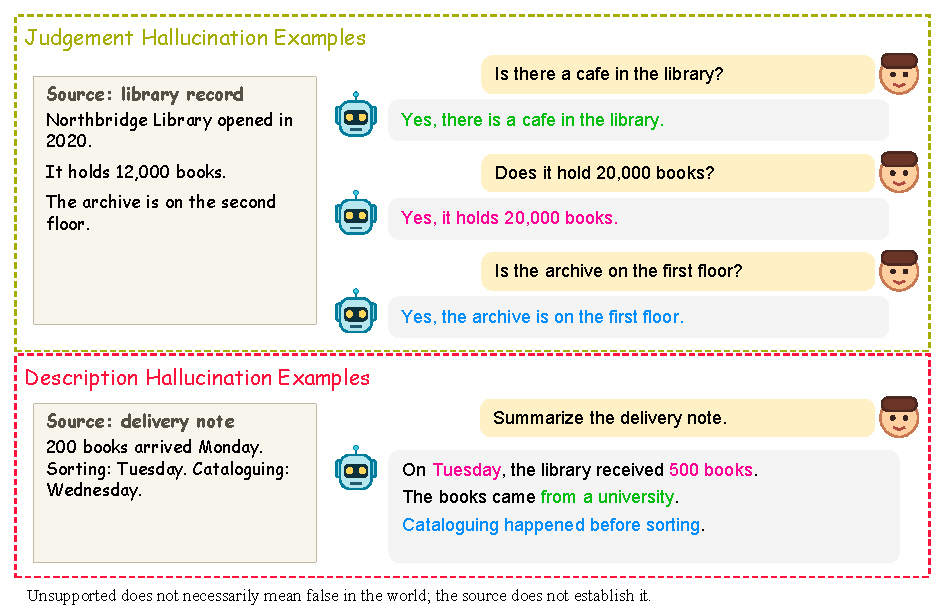
\includegraphics[width=\textwidth]{figures/reference_style/figure_1_hallucination_examples.pdf}
\caption{Source-faithfulness hallucinations in constructed QA and summarization examples, not measured model outputs. Green marks unsupported additions; magenta and blue mark value and relation contradictions. Highlights are illustrative, not an exhaustive taxonomy; world factuality is a separate criterion. Layout adapted from \citet{liu-etal-2024-lvlm-design}.}
\label{fig:hallucination-examples}
\end{figure*}

% First mention: Section 1: closing roadmap, after Figure 1
% These studies are visibly cited inside the vector artwork; register them with BibTeX.
\nocite{cao-etal-2022-hallucinated,dziri-etal-2022-evaluating,adlakha-etal-2024-evaluating,bang-etal-2025-hallulens,wang-etal-2024-factuality,li-etal-2024-dawn,ji-etal-2024-anah,fabbri-etal-2022-qafacteval,zha-etal-2023-alignscore,min-etal-2023-factscore,song-etal-2024-veriscore,harary-etal-2026-prefixnli,manakul-etal-2023-selfcheckgpt,extsemanticuncertainty2023,cohen-etal-2023-lm,zhang-etal-2023-sac3,extsemanticentropy2024,zhang-etal-2023-enhancing-uncertainty,azaria-mitchell-2023-internal,chuang-etal-2024-lookback,liu-etal-2024-universal,fan-etal-2026-refl,lin-etal-2022-truthfulqa,malaviya-etal-2024-expertqa,tang-etal-2024-tofueval,ravichander-etal-2025-halogen,fatahi-bayat-etal-2025-factbench,li-etal-2023-halueval,niu-etal-2024-ragtruth,bao-etal-2025-faithbench,dziri-etal-2022-faithdial,zhang-etal-2024-self,huang-chen-2024-factalign,huang-etal-2025-improving,xue-etal-2025-ualign,jiang-etal-2023-active,zhou-etal-2023-context,extselfrag2024,wang-etal-2025-astute,zhang-etal-2026-stable,shi-etal-2024-trusting,extdola2024,zhang-etal-2024-truthx,wu-etal-2024-synchronous,gema-etal-2025-decore,semnani-etal-2023-wikichat,dhuliawala-etal-2024-chain,extcritic2024,feng-etal-2024-dont,huang-etal-2025-alleviating,godbole-jia-2025-verify,zhao-etal-2025-response,samarinas-etal-2025-beyond,cheang-etal-2026-llms,jiang-etal-2026-benchmarks}
\begin{figure*}[t]
\centering
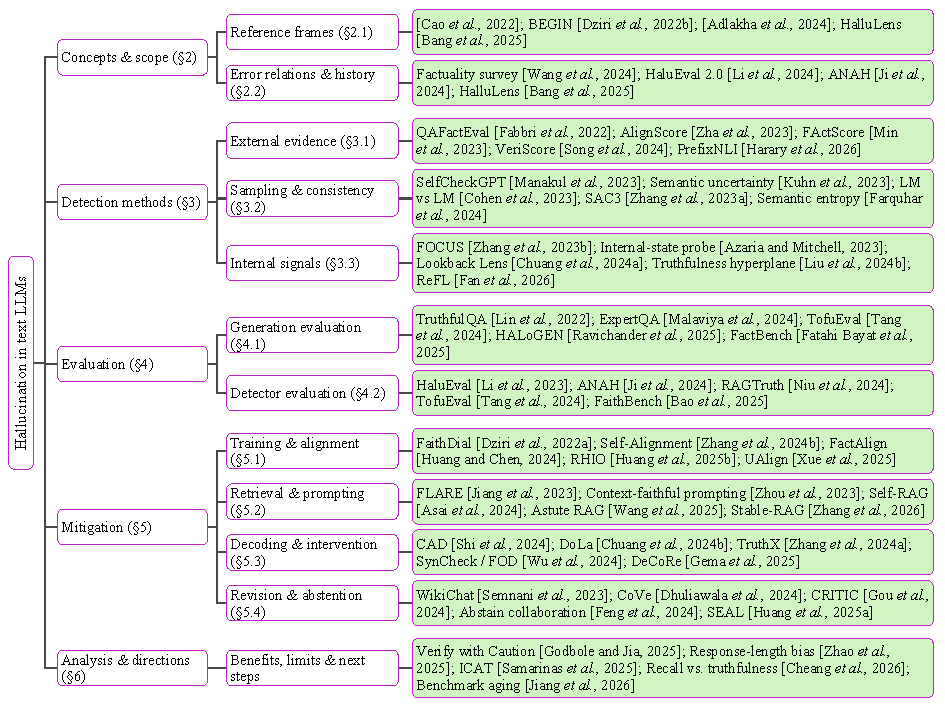
\includegraphics[width=\textwidth]{figures/reference_style/figure_2_survey_structure.pdf}
\caption{The structure of this survey with representative references. Each green leaf includes four to five studies. Evaluation criteria are detailed in Figure~\ref{fig:evaluation-taxonomy} and Table~\ref{tab:hallucination-benchmarks}, and intervention mechanisms in Figure~\ref{fig:causes-mitigation}. Hybrid studies may appear in more than one section. Layout adapted from \citet{liu-etal-2025-logical-design}.}
\label{fig:survey-structure}
\end{figure*}

% First mention: Section 4: evaluation targets; followed by Table 1
% These studies are visibly cited inside the vector artwork; register them with BibTeX.
\nocite{lin-etal-2022-truthfulqa,malaviya-etal-2024-expertqa,ravichander-etal-2025-halogen,fatahi-bayat-etal-2025-factbench,tang-etal-2024-tofueval,bao-etal-2025-faithbench,li-etal-2023-halueval,ji-etal-2024-anah,niu-etal-2024-ragtruth}
\begin{figure*}[t]
\centering
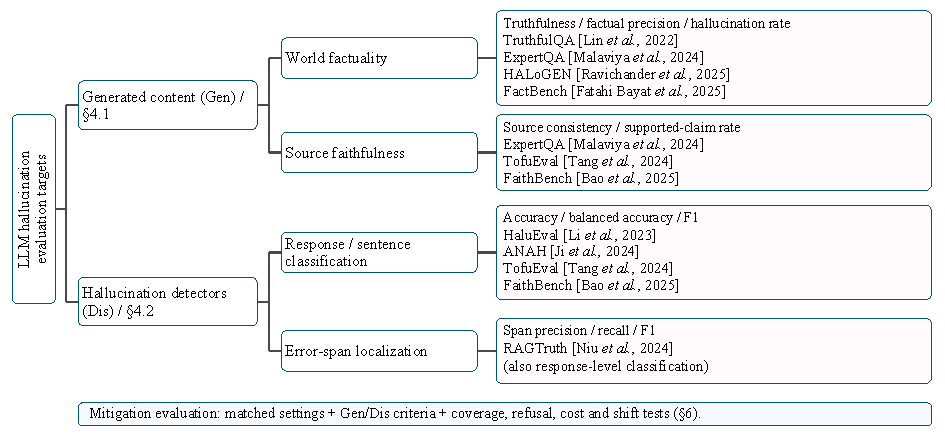
\includegraphics[width=\textwidth]{figures/reference_style/figure_3_evaluation_taxonomy.pdf}
\caption{Taxonomy of evaluation targets and criteria with benchmark references. Gen evaluates generated content; Dis evaluates detectors against human labels. Criteria are not shared protocols; Table~\ref{tab:hallucination-benchmarks} gives benchmark-specific details. The same benchmark may support both targets. Layout adapted from \citet{liu-etal-2024-lvlm-design}.}
\label{fig:evaluation-taxonomy}
\end{figure*}

% First mention: Section 5: mitigation overview; refer back to Section 4
% These studies are visibly cited inside the vector artwork; register them with BibTeX.
\nocite{dziri-etal-2022-faithdial,zhang-etal-2024-self,huang-chen-2024-factalign,extselfrag2024,wang-etal-2025-astute,zhang-etal-2024-truthx,chuang-etal-2024-lookback,shi-etal-2024-trusting,extdola2024,huang-etal-2025-alleviating,dhuliawala-etal-2024-chain,extcritic2024,godbole-jia-2025-verify}
\begin{figure*}[t]
\centering
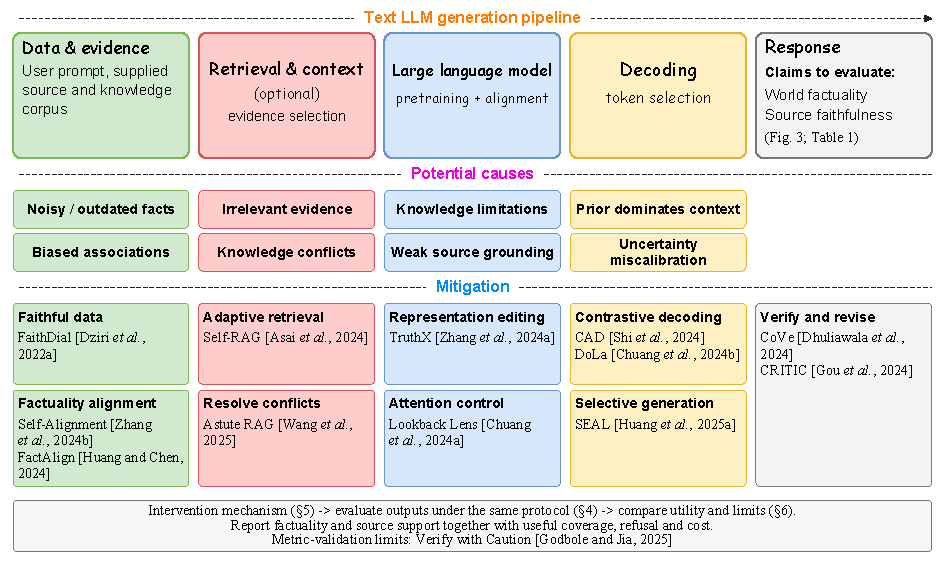
\includegraphics[width=\textwidth]{figures/reference_style/figure_4_causes_mitigation.pdf}
\caption{Potential failure sources and representative mitigation methods in text LLMs. Retrieval is optional. Stage associations summarize the literature; they do not establish one-to-one causal effects or guaranteed fixes. Evaluate outcomes using Figure~\ref{fig:evaluation-taxonomy} and Table~\ref{tab:hallucination-benchmarks}. Layout adapted from \citet{liu-etal-2024-lvlm-design}.}
\label{fig:causes-mitigation}
\end{figure*}
